%
% higherdim.tex -- XXX
%
% (c) 2019 Prof Dr Andreas Mueller
%
\section{Charakteristiken in höheren Dimensionen}
\rhead{Charakteristiken in höheren Dimensionen}
Wir wollen jetzt die Frage nach den Charakteristiken in höheren Dimensionen
stellen. Um die Diskussion überschaubar zu halten, beschränken wir uns auf
das dreidimensionale Problem. Die gefundenen Schlussfolgerungen 
lassen sich sofort auf beliebig viele Dimensionen verallgemeinern.

\subsection{Problemstellung}
Das Cauchy-Problem für eine partielle Differentialgleichung der
Form
\[
\sum_{i,j=1}^3a_{ij}\partial_i\partial_ju+\sum_{i=1}^3b_i\partial_iu+cu=f
\]
besteht darin, dass auf einer Fläche, die zum Beispiel durch
eine Gleichung
\[
\omega(x_1,x_2,x_3)=0
\]
gegeben werden kann,
die Funktionswerte von $u$ vorgegeben werden, sowie die ersten
Ableitungen in eine Richtung senkrecht auf die Fläche.
Diese Ableitung kann mit Hilfe des Gradienten berechnet werden:
\[
\frac{\partial u}{\partial n}=\operatorname{grad}u\cdot \frac{\operatorname{grad}\omega}{|\operatorname{grad}\omega|}
\]
Die Lösung hängt wieder davon ab, ob die Differentialgleichung
und die Anfangsbedingungen die zweiten Ableitungen von $u$ bereits
eindeutig bestimmen.

\subsection{Ein Spezialfall}
Wir betrachten wieder den Spezialfall, in dem die Anfangswerte auf der
Ebene $x_1=0$ vorgegeben sind, also
\begin{align*}
u(0,x_2,x_3)&=u_0(x_2,x_3),
\\
\partial_1u(0,x_2,x_3)&=h(x_2,x_3)
\end{align*}
Dies entspricht dem Fall $\omega(x_1,x_2,x_3)=x_1$.

Durch die Vorgabe der Anfangswerte in Form der Funktion $u_0$ sind die Ableitungen
$\partial_iu$ für $i=2,3$ ebenfalls festgelegt.
Durch Ableiten der Anfangsbedingungen nach $x_2,\dots,x_3$
sind auch die zweiten Ableitungen 
\[
\partial_i\partial_ju(0,x_2,x_3)\qquad 2\le i\le 3,\;1\le j\le 3
\]
bekannt. Es ist also nur noch $\partial_1^2u$ zu bestimmen.
Die Differentialgleichung kann nach $\partial_1^2u$ aufgelöst
werden, wenn $a_{11}\ne 0$. Dies ist gleichbedeutend damit, dass
\[
a_{11}=\begin{pmatrix}
1&0&\dots&0
\end{pmatrix}
A
\begin{pmatrix}1\\0\\\vdots\\0\end{pmatrix}
=0.
\]

\subsection{Der allgemeine Fall}
Wir betrachten die Funktion $\omega(x_1,x_2,x_3)$ als die erste
Koordinaten eines neuen Koordinatensystems. Die Koordinaten in diesem
neuen System nennen wir $\omega_1,\dots,\omega_3$, sie sind Funktionen
der alten Koordinaten
\[
\omega_1(x_1,x_2,x_3)=\omega(x_1,x_2,x_3)
,\qquad
\omega_2(x_1,x_2,x_3)
,\qquad
\omega_3(x_1,x_2,x_3)
\]
Die Funktion $u$ kann natürlich auch in den neuen Koordinaten geschrieben
werden: $\tilde u(\omega_1,\omega_2,\omega_3)$ hat die Eigenschaft
\[
\tilde u(
\omega_1(x_1,x_2,x_3),
\omega_2(x_1,x_2,x_3),
\omega_3(x_1,x_2,x_3)) = u(x_1,x_2,x_3).
\]
Setzt man dies in die Differentialgleichung ein, ergibt sich
\begin{align*}
\partial_iu
&=
\sum_{k=1}^3
\frac{\partial\tilde u}{\partial \omega_k}
\frac{\partial\omega_k}{\partial x_i}
\\
\partial_i\partial_ju
&=
\sum_{k,l=1}^3
\frac{\partial^2\tilde u}{\partial \omega_k\partial\omega_l}
\frac{\partial\omega_k}{\partial x_i}
\frac{\partial\omega_l}{\partial x_j}
\\
\sum_{i,j=1}^3a_{ij}\partial_i\partial_ju
&=
\sum_{i,j,k,l=1}^3a_{ij}
\frac{\partial^2\tilde u}{\partial \omega_k\partial\omega_l}
\frac{\partial\omega_k}{\partial x_i}
\frac{\partial\omega_l}{\partial x_j}
\\
\sum_{i=1}^3b_i\partial_iu
&=
\sum_{i,k=1}^3b_i
\frac{\partial\tilde u}{\partial \omega_k}
\frac{\partial\omega_k}{\partial x_i},
\end{align*}
die Differentialgleichung für $\tilde u$ in den neuen 
Koordinaten lautet also
\[
\sum_{k,l=1}^3a_{ij}
\biggl(
\sum_{i,j=1}^3a_{ij}
\frac{\partial\omega_k}{\partial x_i}
\frac{\partial\omega_l}{\partial x_j}
\biggr)
\frac{\partial^2\tilde u}{\partial \omega_k\partial\omega_l}
+
\sum_{k=1}^3
\biggl(
\sum_{i=1}^3
b_i
\frac{\partial\omega_k}{\partial x_i}
\biggr)
\frac{\partial\tilde u}{\partial \omega_k}
+c\tilde u
=f.
\]
Die neuen Koeffizienten der zweiten Ableitungen sind also
\[
\tilde a_{kl}=
\sum_{i,j=1}^3a_{ij}
\frac{\partial\omega_k}{\partial x_i}
\frac{\partial\omega_l}{\partial x_j}
\]
Die Fläche entspricht in den $\omega$-Koordinaten dem Spezialfall $\omega_1=0$,
die zweiten Ableitungen sind also genau dann eindeutig bestimmt, wenn
der Koeffizient $\tilde a_{11}$ nicht verschwindet. Entlang der durch $\omega$
definierten Fläche sind also genau dann die zweiten Ableitungen nicht eindeutig
bestimmt, wenn 
\[
\sum_{i,j=1}^3
a_{ij}
\frac{\partial\omega}{\partial x_i}
\frac{\partial\omega}{\partial x_j}
=
\operatorname{grad}\omega
\cdot
A
\operatorname{grad}\omega
=0
\]
Da der Gradient senkrecht auf der Fläche steht, also alle Flächen
problematisch, deren Normalen $\vec n$ die Vektorgleichung
\[
\vec n\cdot A\vec n=0
\]
erfüllen. Diese Vektoren heissen {\em charakteristische Normalen}.

\begin{definition}
Eine durch $\omega(x_1,\dots,x_n)=0$ definierte Fläche heisst
charakteristische Fläche, wenn auf der Fläche
\[
\sum_{i,j=1}^na_{ij}\partial_i\omega\partial_j\omega=0
\]
gilt.
\end{definition}

\subsection{Charakteristische Flächen der Wellengleichung}
\begin{figure}
\begin{center}
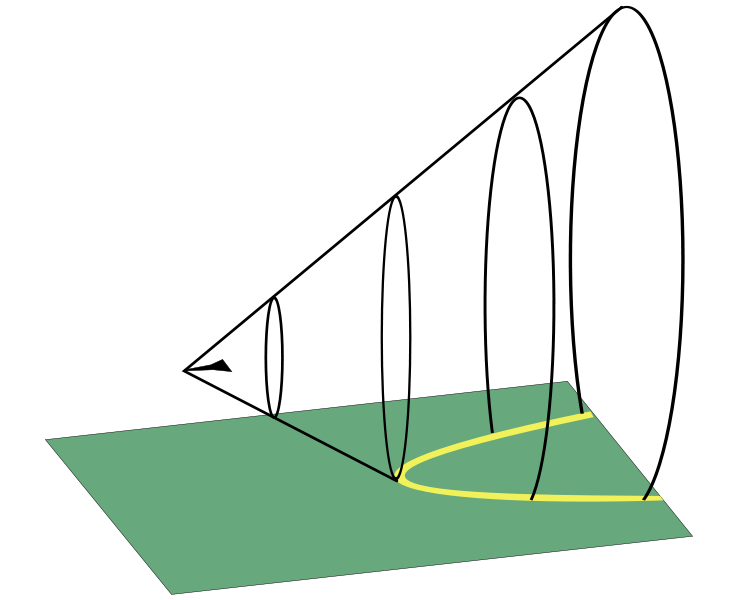
\includegraphics[width=0.8\hsize]{../common/graphics/shock}
\end{center}
\caption{Schockwelle eines Überschallflugzeugs als Beispiel einer
charakteristischen Fläche von $\partial_t^2u-a^2\Delta u=0$.\label{ueberschallkegel}}
\end{figure}
Wir bestimmen die charakteristischen Flächen der
Wellengleichung
\[
\partial_t^2u-a^2\Delta u=0.
\]
Die Koeffizientenmatrix ist
\[
\begin{pmatrix}
1&0&0\\
0&-a^2&0\\
0&0&-a^2
\end{pmatrix},
\]
die charakteristischen Normalen sind also Vektoren $\vec v$, welche die
Gleichung
\[
v_1^2-a^2v_2^2-a^2v_3^2=0
\]
erfüllen. Diese beschreibt einen Doppelkegel, alle Vektoren, welche mit
der $x_1$-Achse einen festen Winkel einschliessen, sind charakteristische
Normalen. Der Winkel $\alpha$ muss der Bedingung
\[
\cos^2\alpha-a^2\sin^2\alpha=0
\]
genügen, also
\[
\tan\alpha=\pm\frac1a.
\]

Die Winkelbedingung ist die einzige Einschränkung an
die charakteristischen Flächen,  entsprechend gibt es eine
grosse Vielfalt:
\begin{enumerate}
\item
Jeder Kegel mit halbem Öffnungswinkel $\frac{\pi}2-\alpha$
und Achse parallel zur $x_1$-Achse ist eine charakteristische Fläche.
Der Kegel schneidet cie $x_2$-$x_3$-Ebene in einem Kreis, dessen Radius mit
grösser werdendem $x_1$ mit der Geschwindigkeit $a$ grösser wird.

Abbildung \ref{ueberschallkegel}
zeigt die Schockwelle eines Überschallflugzeuges. Schockwellen
als Unstetigkeiten müssen sich entlang der charakteristischen Flächen ausbreiten,
also entlang eines Kegels.
\item 
Jede Ebene, die mit der $x_1$-Achse einen Winkel von $\frac\pi2-\alpha$
einschliesst, ist charakteristische Fläche.
Die Ebene schneidet die $x_2$-$x_3$-Ebene in einer Geraden, die sich
mit der Geschwindigkeit $a$ senkrecht zur Geraden fortbewegt.
Diese charakteristische Fläche beschreibt die Fortpflanzung einer
ebenen Welle.
\end{enumerate}


